\chapter{Quantum Computing Programming Languages}
Quantum Programming is assembling quantum programs capable of running on a quantum computer. A Quantum program is used to express quantum algorithms using higher level and much abstract constructs.

\textbf{Quantum Instruction Set} are quantum equivalent of classical Instruction Set Architecture (ISA). They are machine levl 'codes' and are assumed to work on and control funcitonality of ion traps and Qubits. Ion Traps basically control the very very small energy pulses fed to a superconducting chip.\\ 

\section{Quantum Computing SDKs}
\textbf{Quill}\cite{quill} and \textbf{QASM}\cite{qasm} are most referred quantum Instruction Set Architectures. QASM has been made open sourced under the QisKit project by the IBM's Q Experience. The Quantum computing SDKs available now are helpful in running some quantum algorithms on a simulator as well as on hardware system (if you have one). Some examples of commmon one are :

\begin{itemize}
\item{
	\textbf{Project Q}\cite{project_q} is the most recent open sourced project developed by ETH Zurich and it uses python programming to develop quantum logics and circuits. The code produced is either tested on a simulator or run on IBM's Quantum cloud.
}
\item{
	\textbf{QisKit}\cite{qiskit} is the most documented and used project by IBM and is widely used all over the world. It has tutorial that can be accessed here. It's machine implementation uses QASM.
}
\item{
	\textbf{Forest}\cite{forest} project developed by Rigetti, which uses the Python programming language to create and manipulate quantum circuits. Results are obtained either using simulators or prototype quantum devices provided by Rigetti. It uses Quill ISA.
}
\end{itemize}

\section{Imperative QC Languages}
\begin{itemize}
\item{
\textbf{Quantum Computation Language} (QCL)\cite{qcl} is one of the first implemented quantum programming languages. It is an extension of C proggramming language and has support for user defined operators and functions. Its data structure is quite similar to C.
}
\item{
	\textbf{Q language} is the second implemented quantum programming language and it provides conventional class based support for different quantum logic operations. It is complied and tested on a simulator.
}
\item{
	\textbf{QMASM}\cite{QMASM} is a low-level language specific to quantum annealers \footnote{Quantum annealing (QA) is a metaheuristic for finding the global minimum of a given objective function over a given set of candidate solutions (candidate states), by a process using quantum fluctuations.} such as the D-Wave.
}
\end{itemize}

\section{Functional QC Languages}
\begin{itemize}
\item{
\textbf{QML} is a Haskell-like quantum programming language by Altenkirch and Grattage. QML introduces both classical and quantum control operators, whereas most other languages rely on classical control. 
}
\item{
	\textbf{LIQUi$|>$}\cite{liqui} is a quantum simulation extension on the F\# programming language. It is currently being developed by the Quantum Architectures and Computation Group (QuArC) part of the StationQ efforts at Microsoft Research.
}
\end{itemize}

\section{Ongoing Development \& Quantum Stack}
The paper \cite{quantumstack} extensively details about the actual working aspects of a quantum computer. I here by quoting the self explainatory figure used the authors that explain that a quantum computer would essentially be like an external device that will be controlled by a classical computer. The have further explained how the instruction pipelining is being designed and parallelism of Qubits is used.

\begin{figure}[!htb]
\centering
  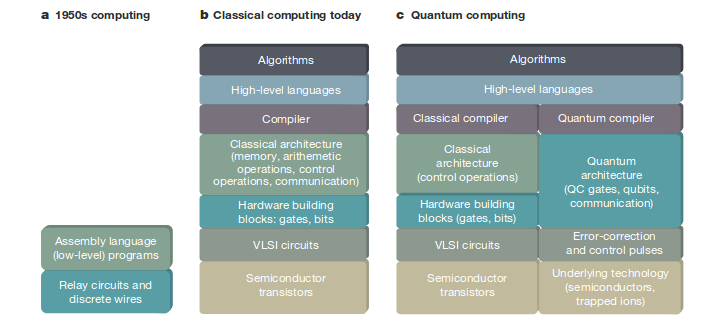
\includegraphics[scale=0.6]{QC_stack}
  \caption{ The different programming stacks (source : The technical paper by Friedric Chong.\protect\cite{quantumstack})}
\end{figure}
